%
% Secção 3.5 Testes
%
\section{Testes}\label{sec35}

\subsection{Testes à Resistência das \textit{Tags} NFC}\label{subsec351}

Existem diferentes condições de conservação para os diversos locais de armazenamento, podendo estes variar em termos de temperatura, humidade, pressão, entre outros. Assim, os alimentos são expostos a circunstâncias distintas aquando armazenados em casa. Por exemplo, no caso dos frigoríficos as capacidades de congelação variam consoante o número de estrelas que possuem, de acordo com a DECO PROTESTE \cite{deco:fridgeStarsClassification}:

\begin{itemize}
    \item 1 estrela: até - 6ºC; conserva congelados até 1 semana.
    \item 2 estrelas: até - 12ºC; conserva congelados até 1 mês.
    \item 3 estrelas: permite conservar alimentos previamente congelados até 1 ano.
    \item 4 estrelas: entre - 18º e - 24ºC; são os únicos que permitem congelar alimentos.
\end{itemize}

O período máximo de conservação de cada alimento varia conforme a classificação de estrelas de um determinado frigorífico/congelador, segundo a DECO PROTESTE \cite{deco:conservationTimeByProduct}. Nos modelos de quatro estrelas os tempos de conservação são os seguintes: 
\begin{itemize}
    \item Frutas e hortícolas cozidas e arrefecidas: 12 meses.
    \item Bifes de vaca sem gordura, salsichas frescas, frango e peru: 10 meses.
    \item Queijos de pasta mole ou semimole: 8 meses.
    \item Pão, massa folhada ou quebrada, bolachas e crepes, manteiga, carne de porco pouco gorda, coelho, lebre e caça, peixe magro ou meio gordo: 6 meses.
    \item Massas para pão e pizzas, tartes de fruta, peixe gordo, marisco, sopas, sobras de pratos cozinhados: 3 meses.
    \item Hambúrgueres, carne picada, carne de porco gorda: 2 meses.
    \item Bolos com creme: 1 mês.
\end{itemize}

Como tal, foi importante testar a resistência das \textit{tags} \acrshort{nfc} às várias condições de conservação, de forma a garantir a eficácia do sistema de gestão de stocks nos diversos espaços de cada casa. Realizaram-se testes em três locais de armazenamento distintos, um frigorífico, um congelador e um armário. Os testes compreenderam a escrita na \textit{tag} e sua arrumação no respetivo local durante um período de tempo estipulado. Após este período de tempo a \textit{tag} foi retirada e verificado o seu estado e ainda retificadas as funcionalidades de leitura e de escrita.

\textbf{Teste às \textit{tags} \acrshort{nfc} no frigorífico:}
\begin{itemize}
\addtolength{\itemindent}{0.5cm} 
    \item Duração: 1 mês
    \item Estrelas: 3
    \item Temperatura: 5 graus Celsius
    \item Humidade: média
    \item Resultado: Leitura e escrita funcionais.
\end{itemize}
     
\textbf{Teste às \textit{tags} \acrshort{nfc} no congelador:}
\begin{itemize}
    \addtolength{\itemindent}{0.5cm} 
    \item Duração: 1 mês
    \item Estrelas: 3
    \item Temperatura: -15 a -18 graus Celsius
    \item Humidade: baixa
    \item Resultado: Leitura e escrita funcionais.
\end{itemize}
    
\textbf{Teste às \textit{tags} \acrshort{nfc} no armário de um quarto de banho:}
\begin{itemize}
    \addtolength{\itemindent}{0.5cm} 
    \item Duração: 1 mês
    \item Temperatura: 15 a 20 graus Celsius
    \item Humidade: alta
    \item Resultado: Leitura e escrita funcionais.
\end{itemize}
   
Em conclusão, para curtos períodos de tempo pode-se garantir a resistência das \textit{tags}, bem como, a eficácia do sistema de gestão de stocks desenvolvido. Contudo, seria imprescindível uma avaliação extensa, com maior gama de períodos de tempo e múltiplas condições, para assim assegurar o sucesso da utilização do sistema Smart Stocks.

\subsection{Testes ao Funcionamento do Sistema Smart Stocks}\label{subsec352}

De forma a poder testar o correto funcionamento do sistema Smart Stocks, simulou-se um dispositivo de hardware por meio de uma aplicação móvel desenvolvida para o propósito. O intuito desta, para além de testar o algoritmo de previsão de stock, é o de simular movimentos, quer sejam de entrada, quer sejam de saída, dos itens numa casa.

Esta aplicação deve ser usada por dispositivos moveis \textit{Android} que suportem a tecnologia \acrshort{nfc} para realizar as leituras das \textit{tags} \acrshort{nfc} e obter a informação do item que está a ser movimentado. De maneira a simular um movimento de entrada ou de saída, existe um \textit{switch} na interface do utilizador que tem o propósito de indicar o tipo do movimento a ser testado. Existe, ainda, a possibilidade de especificar a casa e o identificador do local de armazenamento envolvidos. A aplicação ao ler a informação da \textit{tag}, o tipo de movimento (entrada ou saída), o identificador da casa e do local de armazenamento, envia a informação para a \gls{api-web} e esta irá manusear e armazenar os dados na base de dados.

Com a utilização desta aplicação torna-se fácil testar o algoritmo desenvolvido, pois é apenas necessário realizar movimentos de entrada e saída, num determinado armazenamento de uma determinada casa, para se perceber se algoritmo se encontra a funcionar ou não corretamente, inserindo na lista de compras do sistema Smart Stocks os produtos em vias de acabar.

\subsection{Testes ao Algoritmo de Previsão de Stocks}\label{subsec353}

Afim de testar a implementação do algoritmo de previsão de stocks no sistema Smart Stocks, criou-se um cenário de teste de entradas e saídas de iogurtes numa casa. Analisaram-se as quantidades existentes dos iogurtes, todos os dias às 23h59m durante três semanas. Com estas construiu-se o gráfico abaixo.

Empregando o algoritmo de previsão de stocks desenvolvido obteve-se uma previsão, para a quarta semana, das quantidades de iogurtes previstas para cada dia da semana. De seguida, avalia-se a semana de previsão a fim de se concluir se as quantidades irão descer abaixo de duas unidades, quantidade mínima de segurança utilizada na implementação do algoritmo. Caso tal se verifique, os iogurtes são inseridos na lista de compras, e aí permanecem até a sua quantidade ser igual ou superior ao limite mínimo de segurança. Para calcular a quantidade que é preciso repor, determina-se a distância entre o pico superior e o pico inferior do gráfico. Se estes pontos não existirem, ou seja, apresentarem o mesmo valor, então verifica-se se o mesmo é inferior ao limite de rutura de stock, e calcula-se a diferença a adicionar. 

Posto isto, no caso representado no gráfico deduz-se que dia 25 o número de iogurtes fica abaixo do limite mínimo, pelo que este produto é inserido na lista. Recomenda-se a compra, até esse dia, de pelo menos duas unidades para manter o stock adequado às necessidades previstas para essa semana.

\begin{center}
    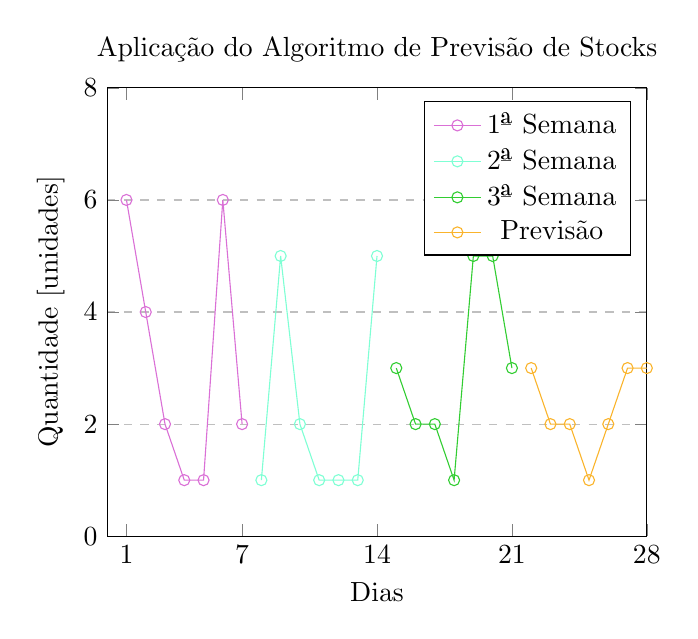
\begin{tikzpicture}
        \begin{axis}[
            title={Aplicação do Algoritmo de Previsão de Stocks},
            xlabel={Dias},
            ylabel={Quantidade [unidades]},
            xmin=0, xmax=28,
            ymin=0, ymax=8,
            xtick={1, 7, 14, 21, 28},
            ytick={},
            legend pos=north east,
            ymajorgrids=true,
            grid style=dashed,
        ]
        \addplot[
            color=Orchid,
            mark=o,
            ]
            coordinates {
            (1,6)(2,4)(3,2)(4,1)(5,1)(6,6)(7,2)
            };
            
        \addplot[
            color=Aquamarine,
            mark=o,
            ]
            coordinates {
            (8,1)(9,5)(10,2)(11,1)(12,1)(13,1)(14,5)
            };
            
        \addplot[
            color=LimeGreen,
            mark=o,
            ]
            coordinates {
            (15,3)(16,2)(17,2)(18,1)(19,5)(20,5)(21,3)
            };
            
        \addplot[
            color=Dandelion,
            mark=o,
            ]
            coordinates {
            (22,3)(23,2)(24,2)(25,1)(26,2)(27,3)(28,3)
            };
            
            \legend{1ª Semana,2ª Semana,3ª Semana,Previsão}
            
        \end{axis}
    \end{tikzpicture}
\end{center}





\subsection{Testes Unitários}\label{subsec354}

Os testes unitários servem para garantir o funcionamento de um componente, por exemplo, se um método funciona, ou seja,  se é retornando o que é esperado, dando garantias ao programador de que a sua aplicação continua a funcionar mesmo após serem efetuadas alterações ou substituídas peças componentes, sendo, assim importante a realização dos testes. 

Estão disponíveis testes unitários para as funções utilitárias. No entanto, a \acrfull{bll} carece de testes. Considerou-se que para realizar estes testes seria necessário demasiado tempo para estes ficarem realmente bem feitos, testando todas as particularidades, como por exemplo, garantir que todas as restrições de integridade estariam a funcionar corretamente, e testando casos em que seria suposto funcionar e noutros que não seria suposto funcionar. A \acrfull{dal} carece também de testes aos métodos desenvolvidos. Os métodos gerados pela \acrshort{jpa} não necessitam de testes uma vez que se confia nessa biblioteca. Para realizar os testes seria necessário simular o acesso à base de dados, usando uma base de dados em memória (\textit{mock}). O \textit{Spring Boot} tem integração com uma base de dados em memória chamada \textit{H2 Database Engine} \cite{H2DatabaseEngine:database}. Esta base de dados será construída com a informação presente nas classes do modelo, as anotações \acrshort{jpa}, pelo que facilitaria simular a base de dados. Contudo a realização destes testes demorariam mais tempo que o disponível para serem realizados da melhor forma.